\documentclass[../main.tex]{subfiles}
\begin{document}
\chapter{Analisi del problema}

\section{Analisi traffico di rete}

Nell'era digitale il traffico di rete è aumentato notevolmente e con esso gli attacchi di tipo informatico, per questo motivo è necessario trovare soluzioni per analizzare questo grande quantitativo di pacchetti che attraversano i dispositivi di rete delle aziende di grosse dimensioni. Nel mondo informatico di oggi è molto importante poter determinare rapidamente e con precisione l'origine e la portata di un potenziale attacco su una rete al fine di poterlo contrastare in modo efficace.
Per fare ciò viene costruito un \textit{audit trail} di informazioni collezionate dal traffico di rete usando una combinazione di network flow e PCAP. 
Un audit trail è un file che contiene una registrazione cronologica di attività relative alla sicurezza per consentire la ricostruzione e l'esame di eventi.

\subsection{Network Flow}
Un flow è una sequenza di pacchetti inviati da una sorgente ad una destinazione che hanno degli attributi in comune:
\begin{itemize}
				\item indirizzo IP sorgente
				\item indirizzo IP destinazione
				\item porta sorgente
				\item porta destinazione
				\item protocollo
\end{itemize}

Se i pacchetti che attraversano un dispositivo di rete hanno questi attributi in comune possono essere raggruppati in un flow.

\subsection{Packet Capture}
Per packet capture (PCAP) si intende la cattura di traffico internet che attraversa un dispositivo di rete. Un packet capture intercetta i singoli pacchetti e li archivia. Nei sistemi operativi Unix è utilizzata la libreria \textbf{libpcap} mentre nei sistemi Windows si fa utilizzo di \textbf{WinPcap}

\subsection{NetFlow}
NetFlow è un protocollo di analisi di rete che offre la possibilità di raccogliere informazioni dettagliate sul traffico mentre attraversa un'interfaccia. NetFlow è una tecnologia proprietaria di Cisco. I dispositivi di rete conformi a NetFlow possono raccogliere statistiche sul traffico ed esportarle come record verso un NetFlow collector, un server che esegue l'analisi del traffico.

Cisco definisce un flow come una sequenza unidirezionale di pacchetti che condividono tutti i seguenti 7 valori:

\begin{itemize}
				\item interfaccia di ingresso
				\item indirizzo IP sorgente
				\item indirizzo IP destinazione
				\item protocollo IP
				\item porta sorgente TCP o UDP, 0 per altri protocolli
				\item IP Type of Service
\end{itemize}

\subsubsection{Componenti di NetFlow}
Una architettura NetFlow ha i seguenti componenti

\begin{figure}[H]
\centering
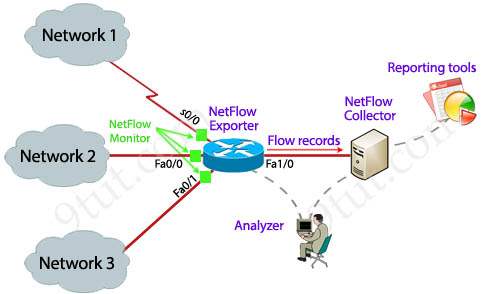
\includegraphics[scale=0.7]{netflowexample.jpg}
\caption{Architettura NetFlow}
\end{figure}

\begin{verse}
\textbf{NetFlow monitor}
un componente applicato a un'interfaccia che raccoglie informazioni sui flow. I NetFlow monitor sono costituiti da un record e una cache.
\end{verse}

\begin{verse}
\textbf{NetFlow exporter}
Aggrega i pacchetti in flows e ne esporta i record verso uno o più \textit{flow collectors}.
Quando dei pacchetti arrivano al NetFlow exporter, vengono ispezionati singolarmente per uno più attributi che vengono utilizzti per determinare se il pachetto è univoco o è simile agli altri pacchetti. Se il pacchetto presenta attributi simili viene classificato nello stesso flow.

\begin{figure}[H]
\centering
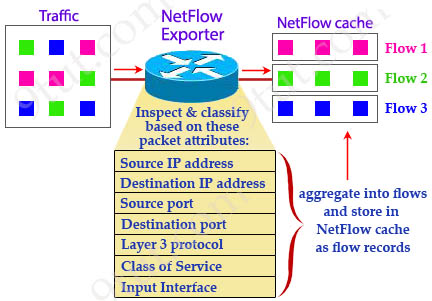
\includegraphics[scale=0.7]{netflowexporter.jpg}
\caption{NetFlow exporter}
\end{figure}

Dopo aver esaminato questi attributi, il NetFlow exporter li aggrega in record di flow e li salva in un database che può essere una cache NetFlow o un NetFlow collector.
\end{verse}

\begin{verse}
\textbf{NetFlow collector}
Responsabile della ricezione, conservazione e pre-elaborazione dei dati di un flow ricevuti da un \textit{flow exporter}. Solitamente è un software separato in esecuzione su un server di rete. I record NetFlow vengono esportati in un NetFlow collector tramite protocollo UDP.
\end{verse}

\begin{verse}
\textbf{Analysis application} 
Analizza i dati dei flows ricevuti nel contesto del rilevamento delle intrusioni o del profilo di traffico.

\begin{figure}[H]
\centering
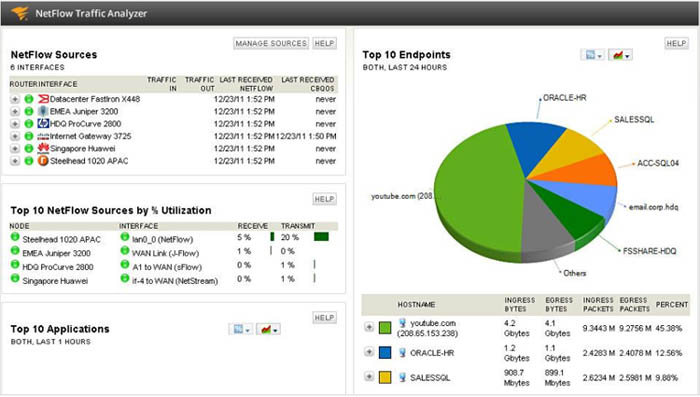
\includegraphics[scale=0.5]{netflowreport.jpg}
\caption{SolarWinds NetFlow Traffic Analyzer}
\end{figure}
\end{verse}


L'analisi dei flow può aiutare a determinare le statistiche del traffico in generale, ma non è sufficiente quando è necessario analizzare una conversazione specifica nel dettaglio. È quindi necessario un utilizzo di entrambe le tecnologie per la monitorazione del traffico.

È importante rendersi conto che una risposta efficae agli incidenti è tutta una questione di dimensioni. Raccogliendo solo PCAP si potrebbero avere troppi dati in un tempo troppo breve, usare PCAP per scoprire con chi uncomputer era connesso su un segmento occupata della rete è, nel migliore dei casi, una lunga query e, nel peggiore dei casi, impossibile (****QUESTO PARAGRAFO VA RISCRITTO****).

Pertanto l'approccio migliore per le organizzazioni è quello di utilizzare prima NetFlow per poi integrarsi con PCAP in un secondo momento.

\section{Strumenti software utilizzati}
Verranno ora descritti i software utilizzati in questa tesi. I software utilizzati sono multipiattaforma, in questa tesi sono stati adoperati su sistema operativo basato su una distribuzione GNU/Linux.

\subsection{Audit Record Generation and Utilization System}
Argus (Audit Record Generation and Utilization System) è la prima implementazione del monitoraggio dei flow, è un progetto open source e multipiattaforma.
Quest'ultima particolarità lo rende molto interessante poichè supportando molti sistemi operativi, trai quali Windows, MaxOSX, Linux, Solaris, FreeBSD, OpenBSD, IRIX e OpenWrt, può essere adoperato in quasi tutte le reti comprendo la maggior parte degli host. La sua architettura è di tipo server/client. Il server recupera i pacchetti ricevuti da una o più interfacce di rete disponibili su una una macchina, argus assembla poi questi pacchetti in dati binari che rappresentano dei flow. Lo scopo dei client è di quello di leggere i dati dei flow. \newline

Argus viene utilizzato da molte università e aziende per registrare dei flow che vengono utilizzati sia nell'analisi immediata dell'utilizzo della rete, sia nell'analisi storica.
I record Netflow di Argus offrono un rapporto fino a 10.000:1 dalla dimensione del pacchetto al record scritto sul disco, che consente alle installazioni di salvare i record per molto più tempo rispetto alle acquisizioni di pacchetti completi.


\begin{table}[h]
\begin{tabular}{|l|l|}
\hline
\textbf{campo} & \textbf{descrizione}                    \\ \hline
StartTime      & record start time                       \\ \hline
Dur            & record total duration                   \\ \hline
Proto          & transaction protocol                    \\ \hline
SrcAddr        & source IP address                       \\ \hline
Sport          & source port number                      \\ \hline
Dir            & direction of transaction                \\ \hline
DstAddr        & destination IP address                  \\ \hline
Dport          & destination port number                 \\ \hline
State          & transaction state                       \\ \hline
sTos           & source TOS byte value                   \\ \hline
dTos           & destination TOS byte value              \\ \hline
TotPkts        & total transaction packet count          \\ \hline
TotBytes       & total transaction bytes                 \\ \hline
SrcBytes       & src -\textgreater dst transaction bytes \\ \hline
srcUdata       & source user data buffer                 \\ \hline
dstUdata       & destination user data buffer            \\ \hline
Label          & metadata label                          \\ \hline
\end{tabular}
\end{table}

\section{nProbe}

Negli ambienti commerciali, NetFlow è probabilmente lo standard de facto per la contabilità e la fatturazione del traffico di rete. nProbe è un software in grado di reccogliere, analizzare ed esportare report sul traffico di rete utilizzando il formato standard Cisco NetFlow. È disponibile per la maggior parte dei sistemi operativi sul mercato. \newline

Nel monitoraggio basato sui flow ci sono due componenti principali: il flow exporter e il flow collector. Solitamente NetFlow è un pradigma in modalità push poichè i dispositivi di rete non hanno quasi nessun tipo di memoria di archiviazione e quindi inviano i dai il più presto possibile verso un collector. Questa architettura non è ottimale poichè la sonda sta inviando gli stessi dati a tutti i collector e anche perchè nel caso in cui debba essere aggiunto un nuovo collector, la sonda deve essere riconfigurata. Un altro problema è che i dati scambiati sono in chiaro, il che significa che chiunque intercetta i flussi inviati dalla sonda può scoprire cosa succede nella rete monitorata. 
Ntopng ha ripristinato questo paradigma utilizzando un'architettura in modalità polling. \newline

Con l'utilizzo di ZMQ ntopng si iscrive in modo dinamico alla sonda, comunica alla sonda il tipo di dati a cui è interessata nel flow e la sonda invia solo questa informazione, senza inviare tutti i flow a ntopng. Questa pratica ottimizza il traffico di rete e limita i cicli della CPU a quelli realmente necessari per continuare a raccogliere flows.

\paragraph{ZeroMQ}
ZeroMQ è una libreria di messagistica asincrona ad alte prestazione destinata all'utilizzo in applicazioni distribuite o concorrenti. L'API ZeroMQ fornisce socket che possono rappresentare una connessione molti-a-molti tra endpoint. Operando con una granularità del messaggio, richiedono l'uso di un pattern di messagistica e sono particolarmente ottimizzati per quel tipo di pattern.


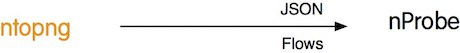
\includegraphics[scale=1.5]{PollMode.jpg}{H}



\begin{table}[h]
\begin{tabular}{|l|l|}
\hline
\multicolumn{1}{|c|}{\textbf{campo}} & \multicolumn{1}{c|}{\textbf{descrizione}}     \\ \hline
IPV4\_SRC\_ADDR                      & IPv4 source address                           \\ \hline
IPV4\_DST\_ADDR                      & IPv4 destination address                      \\ \hline
IPV4\_NEXT\_HOP                      & IPv4 next hop address                         \\ \hline
INPUT\_SNMP                          & input interface SNMP idx                      \\ \hline
OUTPUT\_SNMP                         & output interface SNMP idx                     \\ \hline
IN\_PKTS                             & incoming flow packets (src -\textgreater dst) \\ \hline
IN\_BYTES                            & incoming flow bytes (src -\textgreater dst)   \\ \hline
FIRST\_SWITCHED                      & SysUptime (msec) of the first flow pkt        \\ \hline
LAST\_SWITCHED                       & SysUptime (msec) of the last flow pkt         \\ \hline
L4\_SRC\_PORT                        & IPv4 source port                              \\ \hline
L4\_DST\_PORT                        & IPv4 destination port                         \\ \hline
TCP\_FLAGS                           & cumulative of all flow TCP flags              \\ \hline
PROTOCOL                             & IP protocol byte                              \\ \hline
SRC\_TOS                             & Type of service byte                          \\ \hline
SRC\_AS                              & source BGP AS                                 \\ \hline
DST\_AS                              & destination BGP AS                            \\ \hline
IPV4\_SRC\_MASK                      & IPv4 source subnet mask                       \\ \hline
IPV4\_DST\_MASK                      & IPv4 dest subnet mask                         \\ \hline
L7\_PROTO                            & layer 7 protocol (numeric)                    \\ \hline
BIFLOW\_DIRECTION                    & 1=initiator, 2=reverseInitiator               \\ \hline
FLOW\_START\_SEC                     & seconds (epoch) of the first flow packet      \\ \hline
FLOW\_END\_SEC                       & seconds (epoch) of the last flow packet       \\ \hline
OUT\_PKTS                            & outgoing flow packets (dst -\textgreater src) \\ \hline
OUT\_BYTES                           & outgoing flow bytes (dst -\textgreater src)   \\ \hline
FLOW\_ID                             & serial flow identifier                        \\ \hline
FLOW\_ACTIVE\_TIMEOUT                & activity timeout of flow cache entries        \\ \hline
FLOW\_INACTIVE\_TIMEOUT              & inactivity timeout of flow cache entries      \\ \hline
IN\_SRC\_MAC                         & source MAC address                            \\ \hline
OUT\_DST\_MAC                        & destination MAC address                       \\ \hline
\end{tabular}
\end{table}

\section{Stratosphere IPS}
In questa tesi si è utilizzato Stratosphere Testing Framework, un \textit{Network Intrusion Detection System} che genera modelli comportamentali delle connessioni di reti. Il suo obiettivo è aiutare i ricercatori a trovare nuovi comportamenti malware, etichettare tali comportamenti, creare i loro modelli di traffico e verificare gli algoritmi di rilevamento. Stf funziona utilizzando algoritmi di apprendimento automatico sui modelli comportamentali.

L'obiettivo di Stratosphere Project è quello di creare un \textit{IDS} comportamentale in grado di rilevare e bloccare i comportamenti dannosi nella rete.

Come parte di questo progetto, stf viene utilizzato per generare modelli altamente attendibili di traffico dannoso consentendo una verifica automatica delle prestazioni di rilevamento. \newline

\textit{Stratosphere IPS} non è strettamente un \textit{IPS} nel senso che può impedire l'intrusione. Usa l'acronimo \textit{IPS} perchè l'\textit{IPS} di Stratosphere può bloccare connessioni malevoli usando il firewall del computer. Tuttavia, a causa della natura delle connessioni di traffico, l'\textit{IPS} di Stratosphere necessita di un po' di tempo per rilevare il comportamento dannoso e quindi non può bloccare i primi pacchetti nella connessione.

L'\textit{IPS} di Stratosphere è in grado di rilevare e bloccare connessioni di rete molto fini e pericolose, e quindi dovrebbe essere visto come un complemento delle attuali misure di sicurezza della rete.

\subsection{Il significato dei modelli comportamentali} 
Il nucleo di \textit{Stratosphere IPS} è composto dai modelli comportamentali di reti e algoritmi di rilevamento. I modelli comportamentali rappresentano ciò che una connessione specifica fa nella rete durante la sua vita. Il comportamento è costuito analizzando la sua periodicità, le dimensioni e la durata di ciascun flusso. Sulla base di queste caratteristiche a ciascun flusso viene assegnata una lettera e il gruppo di lettere caratterizza il comportamento della connessione.

Prendiamo come esempio una connessione generata da una botnet che ha il seguente modello comportamentale
\begin{lstlisting}[language=bash]
88*y*y*i*H*H*H*y*0yy*H*H*H*y*y*y*y*H*h*y*h*h*H*H*h*H*y*y*y*H*
\end{lstlisting}

Questa catena di stati che chiamiamo modello comportamentale evidenzia alcune delle caratteristiche del canale C\&C. In questo caso ci dice che i flussi sono altamente periodici (lettere \textit{h}, \textit{i}), con qualche periodicità persa vicino all'inizio (lettere \textit{y}). I flussi hanno anche una grande dimensione con una durata media. I simboli tra le lettere sono correlati al tempo trascorso tra i flussi. In questo caso il simbolo '\textit{*}' significa che il flusso è separato da meno di un'ora. Guardando le lettere si può vedere che questa è una connessione piuttosto periodica, e controllando efficacemente i suoi flussi confermiamo tale ipotesi.
Con l'utilizzo di questo tipo di modelli siamo in grado di generare le caratteristiche comportamentali di un gran numero di azioni dannose. L'immagine seguente mostra i criteri di assegnazione delle lettere per i modelli comportamentali \newline
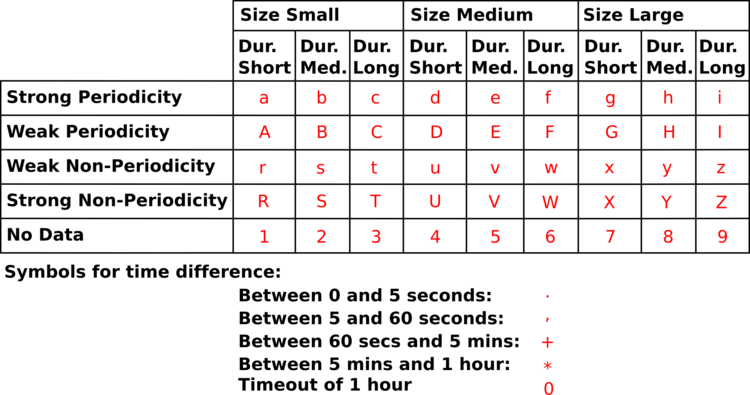
\includegraphics[scale=0.5]{modello-comportamentale.png}


Gli algoritmi di rilevamento utilizzano modelli comportamentali proprietari dannosi per rilevare nuove connessioni sospette nella rete. Il rilevamento viene attualmente eseguito utilizzando algoritmi basati su catene di \textit{Markov}.
La prima parte dell'algoritmo consiste nell'apprendimento e nell'etichettatura del traffico di verità di base. Questo traffico viene utilizzato per creare modelli verificati di comportamenti di rete noti e stabili. \newline

La seconda parte dell'algoritmo consiste nell'utilizzare questi modelli di verità di base noti e verificati per rilevare comportamenti simili in reti sconosciute. \textit{Stratosphere IPS} catturerà il traffico in un computer client e confronterà ogni connessione sconosciuta con i modelli conosciuti di comportamento del traffico. Poichè il modo in cui viene effettuato il rilevamento e come vengono creati i modelli, ciascun modello comportamentale può corrispondere a un'ampia gamma di comportamenti simili senza essere troppo generico. I modelli sono quindi utili per trovare comportamenti simili senza il rischio di generare troppi falsi positivi.


\section{Problematiche dovute all'utilizzo di due diversi formati}
Come si è potuto notare nelle sezioni \textit{2.2} e \textit{2.3}, gli header di \textit{nProbe} ed \textit{Argus} presentano delle differenze che non permettono di essere utilizzati in modo intercambiabile. I file che produce in output \textit{Argus} presentano 17 cambi, ben 12 in meno rispetto ai file di output prodotti da \textit{nProbe}.
L'utilizzazione di due diversi formati presenta errori quando si cerca di utilizzare file prodotti da \textit{nProbe} in Stratosphere IPS. \newline

Questa incompatibilità ha portato alla necessità di una conversione: i file prodotti dal \textit{DIEF} devono essere convertiti in file di formato usato da \textit{Argus}. Questa conversione deve essere efficiente e precisa.

\section{Presentazione del problema}
Il \textit{DIEF} salva i file in una struttura gerarchica fissa ben definita: ci sono 4 livelli di subdir, in cui il primo livello indica l'anno, il secondo il mese, il terzo il giorno e il quarto l'ora. All'interno dell'ultima subdir, quella delle ore, ci sono 60 file uno per ogni minuto della giornata.

\begin{forest}
  for tree={
    font=\ttfamily,
    grow'=0,
    child anchor=west,
    parent anchor=south,
    anchor=west,
    calign=first,
    inner xsep=7pt,
    edge path={
      \noexpand\path [draw, \forestoption{edge}]
      (!u.south west) +(7.5pt,0) |- (.child anchor) pic {folder} \forestoption{edge label};
    },
    before typesetting nodes={
      if n=1
        {insert before={[,phantom]}}
        {}
    },
    fit=band,
    before computing xy={l=15pt},
  }  
[folder structure
  [years
    [months
        [days
            [hours]
        ]
    ]
  ]
]
\end{forest} \newline \newline

I file dei minuti sono compressi usando il programma \textit{gzip}, pertanto c'è da tenerne conto nella soluzione per la conversione.
\end{document}
